\pagebreak
\section{Analisi dei requisiti}
\label{sez:analisi-dei-requisiti}
L’analisi dei requisiti rappresenta una fase cruciale in qualsiasi progetto \textit{software}, poiché consente di definire in modo dettagliato e strutturato ciò che il sistema dovrà realizzare per soddisfare le necessità degli utenti e degli \textit{stakeholder}.\\
In questo progetto, l’analisi è stata condotta seguendo un approccio metodico che si è articolato in diverse fasi.\\

\noindent In primo luogo, ho effettuato una mappatura delle \gls{user-stories}, un processo che ha permesso di identificare le funzionalità principali richieste dagli utenti attraverso una rappresentazione visuale e iterativa. \\
Successivamente, ho individuato i casi d’uso, descrivendo in dettaglio gli scenari di interazione tra gli attori del sistema e le funzionalità del \textit{software}.\\
Infine, sulla base di queste informazioni, ho creato i \textit{requisiti}, formalizzando in modo chiaro e specifico ciò che il sistema deve implementare, suddividendo i requisiti in funzionali e non funzionali per garantire una visione completa del progetto.
\subsection{\textit{User Story Mapping}}
\label{subsec:user-story-mapping}

\subsection*{Introduzione}
\label{subsubsec:introduzione}

Le \gls{user-stories} rappresentano una tecnica fondamentale nel contesto dello sviluppo \textit{Agile}, in particolare all'interno del \textit{framework} \textit{Scrum}. \\
Questa metodologia consente di creare una visione d'insieme delle funzionalità richieste da un sistema, organizzandole in modo strutturato e collaborativo\footcite{site:user-stories}. \\

\noindent Lo \textit{User Story Mapping} è uno strumento visuale che suddivide il lavoro in componenti incrementali, aiutando il \textit{team} a comprendere il percorso del cliente e a pianificare il rilascio di valore progressivo.\\

\subsection*{Utilizzo nel contesto \textit{Scrum}}\\

\noindent Nel contesto di \textit{Scrum}, le \gls{user-stories} sono utilizzate per:

\begin{itemize}
    \item \textbf{Comprendere le esigenze degli utenti:} La mappatura aiuta a identificare le principali funzionalità del prodotto dal punto di vista degli utenti finali;
    \item \textbf{Definire un \textit{backlog} strutturato:} La tecnica consente di creare un \gls{product-backlog} organizzato, ordinando le \gls{user-stories} per priorità e obiettivi di rilascio;
    \item \textbf{Pianificare gli \gls{sprint}:} La mappa aiuta il \textit{Product Owner} ed il \textit{team} ad individuare le storie da completare in ciascun \gls{sprint}, bilanciando valore e complessità;
    \item \textbf{Favorire la collaborazione:} La mappa è creata in un incontro collaborativo che coinvolge il \textit{Product Owner}, il \textit{team} di sviluppo e, quando possibile, gli \textit{stakeholder}, per garantire un allineamento sulle priorità.
\end{itemize}

\pagebreak
\subsection*{Struttura delle \gls{user-stories}}\\

\noindent Ogni \textit{user story} segue una struttura standard che include diversi elementi essenziali:\\
\begin{itemize}

    \item \textbf{Priorità}, ogni storia viene classificata in base alla sua priorità, indicata con tre livelli derivati dal metodo \textit{MoSCoW}\footcite{site:moscow-method}:
    \begin{itemize}
        \item \textbf{M:} \textit{Must have} (essenziale): funzionalità indispensabili per il sistema;
        \item \textbf{S:} \textit{Should have} (importante): funzionalità utili ma non critiche;
        \item \textbf{C:} \textit{Could have} (opzionale): funzionalità che aggiungono valore ma possono essere escluse in caso di limitazioni temporali o di risorse.   
    \end{itemize}

    \item \textbf{Descrizione}, ogni storia è descritta in modo sintetico attraverso la notazione standard:

    \begin{center}
        Come [\textit{utente}], voglio [\textit{azione}], affinché [\textit{obiettivo}].
    \end{center}
    Ad esempio: "Come cliente, voglio visualizzare il catalogo prodotti, affinché possa scegliere cosa acquistare."\\

    \item \textbf{Criteri di accettazione}, questi definiscono le condizioni che devono essere soddisfatte affinché le \gls{user-stories} possano essere considerate completate.\\
    Sono specifiche misurabili che servono come riferimento per i \textit{test} e l’approvazione. \\

    \noindent Ad esempio, per la storia sopra, i criteri di accettazione potrebbero essere:

    \begin{itemize}
        \item Il catalogo deve mostrare almeno 20 prodotti per pagina;
        \item Ogni prodotto deve avere nome, immagine e prezzo visibili;
        \item L’utente deve poter filtrare i prodotti per categoria.
    \end{itemize}

\end{itemize}

\noindent Questa combinazione di priorità, descrizione e criteri di accettazione rende le \gls{user-stories} uno strumento potente per pianificare, monitorare e validare lo sviluppo di un progetto, assicurando che tutte le funzionalità siano orientate al valore per l’utente e il \textit{business}.

\pagebreak
\subsection*{\textit{Epic} e \textit{stories} identificate}
\label{subsubsec:epic-stories}

\vspace{0.5cm}
\section*{\textit{Epic} 1: Accesso alla piattaforma}

\subsection*{\textbf{M} - \textit{Login} nel sistema:}

\noindent Come utente voglio poter accedere al sistema e visualizzare la \textit{dashboard} così da gestire i miei progetti precedenti e crearne di nuovi. 

\subsubsection*{Criteri di accettazione:}

\begin{enumerate}
    \item L'utente deve poter accedere inserendo \textit{email} e \textit{password};
    \item In caso di credenziali corrette, l'utente deve essere reindirizzato alla \textit{dashboard} personale;
    \item Se le credenziali sono errate, deve essere mostrato un messaggio di errore appropriato;
    \item Il sistema deve rispettare le politiche di sicurezza, come il blocco temporaneo dopo tentativi falliti ripetuti.
\end{enumerate}

\vspace{0.5cm}

\subsection*{M - Errore di accesso in caso di credenziali errate:}

\noindent Come utente in caso di errore di accesso (es. \textit{password} errata), voglio essere informato con un messaggio chiaro su come risolvere il problema (ad es. come reimpostare la \textit{password}).

\subsubsection*{Criteri di accettazione:}

\begin{enumerate}
    \item Deve essere visualizzato un messaggio chiaro con istruzioni per risolvere il problema (ad esempio, come reimpostare la \textit{password});
    \item Il messaggio di errore non deve rivelare se l'\textit{email} esiste nel sistema per motivi di sicurezza.
\end{enumerate}

\vspace{0.5cm}
\subsection*{M - Piattaforma ottimizzata per \textit{mobile}:}

\noindent Come utente voglio poter accedere alla piattaforma \textit{web} tramite un'interfaccia \textit{mobile} ottimizzata così da poter gestire i miei progetti con facilità anche in mobilità.

\subsubsection*{Criteri di accettazione:}

\begin{enumerate}
    \item La piattaforma deve essere accessibile tramite \textit{browser mobile};
    \item Tutte le funzionalità chiave devono essere usabili su uno schermo \textit{mobile} senza problemi di \textit{layout} o navigazione.
\end{enumerate}

\vspace{0.5cm}

\subsection*{M - \textit{Logout }dal sistema:}

\noindent Come utente voglio avere la possibilità di disconnettermi dal sistema in modo semplice e rapido, così da garantire la sicurezza del mio \textit{account} e prevenire accessi non autorizzati.

\subsubsection*{Criteri di accettazione:}

\begin{enumerate}
    \item L'utente deve potersi disconnettere tramite un pulsante di \textit{logout} ben visibile;
    \item Dopo il \textit{logout}, l'utente deve essere reindirizzato alla pagina di \textit{login};
    \item La sessione dell'utente deve essere invalidata immediatamente.
\end{enumerate}

\vspace{0.5cm}

\section*{\textit{Epic} 2: Gestione dei Progetti}

\subsection*{S - Funzione ricerca e filtraggio progetti:}

\noindent Come utente voglio poter cercare e filtrare i miei progetti per data o nome così da trovare facilmente il progetto desiderato anche in un elenco molto lungo. 

\subsubsection*{Criteri di accettazione:}

\begin{enumerate}
    \item L'utente deve poter cercare i progetti per nome o data tramite un campo di ricerca;
    \item I risultati devono essere aggiornati dinamicamente durante la ricerca;
    \item I filtri devono includere opzioni per ordinare per data di creazione o nome.
\end{enumerate}

\vspace{0.5cm}

\subsection*{M - Visualizzazione singolo progetto}

\noindent Come utente voglio poter selezionare un singolo progetto salvato nella \textit{dashboard} così da visualizzarne i dettagli (nome, stato, data di creazione e le ultime modifiche) e poterlo rigenerare. 

\subsubsection*{Criteri di accettazione:}

\begin{enumerate}
    \item L'utente deve poter cliccare su un progetto dalla lista per accedere alla sua vista dettagliata;
    \item La pagina del progetto deve mostrare nome, stato, data di creazione e tutti i capitoli generati;
    \item Deve essere presente un'opzione per rigenerare il progetto dalla pagina di dettaglio dello stesso.
\end{enumerate}

\vspace{0.5cm}

\subsection*{M - Visualizzazione lista progetto:}

\noindent Come utente voglio poter vedere la lista di tutti i progetti precedentemente generati con annesso nome e data creazione, così da poter scegliere quale selezionare. 

\subsubsection*{Criteri di accettazione:}

\begin{enumerate}
    \item Tutti i progetti dell'utente devono essere visibili in una lista con nome e data di creazione:
    \item La lista deve essere scorrevole e ottimizzata per schermi di diverse dimensioni.
\end{enumerate}

\vspace{0.5cm}

\subsection*{M - Rigenerazione di un progetto:}

\noindent Come utente voglio poter rigenerare un progetto, aggiungendo o modificando informazioni, così da ottenere diverse versioni del documento per meglio adattarsi alle mie esigenze.

\subsubsection*{Criteri di accettazione:}

\begin{enumerate}
    \item L'utente deve poter accedere alla funzione di rigenerazione da un progetto esistente;
    \item Deve essere possibile inserire un \gls{prompt} contenente le direttive da usare per la rigenerazione del progetto;
    \item La versione rigenerata deve essere salvata come nuova versione del progetto.
\end{enumerate}

\vspace{0.5cm}

\subsection*{C - Visualizzazione versioni precedenti progetto:}

\noindent Come utente voglio poter visualizzare le versioni precedenti di un progetto così da poter ripristinare o confrontare modifiche, migliorando il controllo sulle evoluzioni del documento.

\subsubsection*{Criteri di accettazione:}

\begin{enumerate}
    \item L'utente deve poter visualizzare una lista cronologica delle versioni precedenti del progetto;
    \item Deve essere possibile selezionare e visualizzare una versione precedente.
\end{enumerate}

\vspace{0.5cm}
\pagebreak
\subsection*{S - Rigenerazione specifici capitoli}

\noindent Come utente voglio rigenerare specifici capitoli di un progetto già creato, mantenendo inalterati gli altri capitoli, così da aggiornare solo le sezioni che richiedono modifiche senza dover rigenerare tutto il documento.

\subsubsection*{Criteri di accettazione:}

\begin{enumerate}
    \item L'utente deve poter selezionare il capitolo da rigenerare dalla pagina di visualizzazione singolo progetto;
    \item Deve essere possibile inserire un \gls{prompt} contenente le direttive da usare per la rigenerazione del capitolo;
    \item La versione rigenerata deve essere salvata come nuova versione del progetto;
    \item I capitoli non selezionati devono rimanere invariati.
\end{enumerate}

\vspace{0.5cm}

\subsection*{C - Rimozione capitoli non necessari:}

\noindent Come utente voglio poter rimuovere singoli capitoli così da eliminare contenuti non necessari dal progetto. 

\subsubsection*{Criteri di accettazione:}

\begin{enumerate}
    \item L'utente deve poter selezionare e rimuovere i capitoli dal progetto;
    \item Prima della rimozione definitiva, deve essere mostrata una finestra di conferma.
\end{enumerate}

\vspace{0.5cm}

\subsection*{M - Eliminazione di un progetto:}

\noindent Come utente, voglio poter eliminare un progetto che ho creato in modo che possa rimuovere progetti non più necessari o irrilevanti.

\subsubsection*{Criteri di accettazione:}

\begin{enumerate}
    \item L'utente dalla pagina di visualizzazione singolo progetto deve poter richiedere l’eliminazione dello stesso;
    \item Deve essere mostrata una finestra di conferma prima dell'eliminazione definitiva del progetto;
    \item L'eliminazione deve rimuovere tutti i dati associati al progetto senza lasciare tracce;
    \item Se l'eliminazione è completata con successo, l'utente deve ricevere una notifica di conferma.
\end{enumerate}

\vspace{0.5cm}

\section*{\textit{Epic} 3: Creazione di nuovi progetti}

\subsection*{M - Generazione progetto tramite \textit{preset}:}

\noindent Come utente voglio poter generare un progetto con l'aiuto di \textit{preset} predefiniti e ottimizzati, così da creare rapidamente un documento utile e strutturato senza partire da zero.

\subsubsection*{Criteri di accettazione:}

\begin{enumerate}
    \item All’interno della pagina di creazione di un progetto l'utente deve poter selezionare un \textit{preset} predefinito dalla lista;
    \item Dopo la selezione e la compilazione del \textit{preset} il progetto deve essere generato con i dati inseriti;
    \item Se la generazione avviene con successo, l’utente viene reindirizzato alla pagina di visualizzazione del singolo progetto;
    \item L’utente riceve una notifica di successo.
\end{enumerate}

\vspace{0.5cm}

\subsection*{M - Visualizzazione descrizione \textit{preset}:}

\noindent Come utente voglio visualizzare una descrizione dettagliata di ciascun \textit{preset} così da scegliere quello più adatto alle mie esigenze specifiche.

\subsubsection*{Criteri di accettazione:}

\begin{enumerate}
    \item Ogni \textit{preset} deve avere una descrizione dettagliata visibile prima della selezione;
    \item La descrizione deve includere le caratteristiche e i casi d'uso principali del \textit{preset}.
\end{enumerate}

\vspace{0.5cm}

\subsection*{S - Salvataggio \textit{preset} compilato:}

\noindent Come utente voglio poter salvare il \textit{preset} compilato così da poterlo completare e generare il documento in un momento successivo.

\subsubsection*{Criteri di accettazione:}

\begin{enumerate}
    \item L'utente deve poter salvare un \textit{preset} (parzialmente) compilato per completarlo in un secondo momento;
    \item Il sistema deve indicare chiaramente che il \textit{preset} è salvato in bozza.
\end{enumerate}

\vspace{0.5cm}

\pagebreak
\subsection*{C - Personalizzazione campi \textit{preset}:}

\noindent Come utente voglio personalizzare i campi del \textit{preset} così da adattarlo alle mie specifiche necessità e rendere unico il progetto. 

\subsubsection*{Criteri di accettazione:}

\begin{enumerate}
    \item L'utente deve poter modificare i campi predefiniti del \textit{preset};
    \item Le modifiche devono essere salvate, rendendo possibile l’utilizzo del \textit{preset} personalizzato in secondo momento
\end{enumerate}

\vspace{0.5cm}

\subsection*{C - Generazione progetto senza \textit{preset}:}

\noindent Come utente voglio poter generare un progetto senza l’utilizzo di un \textit{preset} così da avere il massimo controllo e flessibilità sulla struttura del documento finale, migliorando la personalizzazione per casi d'uso complessi. 

\subsubsection*{Criteri di accettazione:}

\begin{enumerate}
    \item L'utente deve poter generare un nuovo progetto senza scegliere un \textit{preset};
    \item Deve essere possibile inserire un prompt contenente le direttive da usare per la generazione del progetto.
\end{enumerate}

\vspace{0.5cm}

\subsection*{M - Download documento progetto:}

\noindent Come utente voglio poter scaricare il progetto generato in formato PDF così da poterlo condividere facilmente con il mio \textit{team} o archiviare per un utilizzo futuro.

\subsubsection*{Criteri di accettazione:}

\begin{enumerate}
    \item Dalla pagina di visualizzazione singolo progetto l'utente deve poter scaricare il progetto in formato PDF;
    \item Il \textit{file} generato deve includere tutti i capitoli del progetto.
\end{enumerate}

\vspace{0.5cm}

\subsection*{S - Generazione progetto tramite diversi \gls{llm}:}

\noindent Come utente voglio poter scegliere tra vari \gls{llm} per la generazione del progetto così da avere varie maggiore scelta (progetti più grandi vs. progetti più piccoli). 

\subsubsection*{Criteri di accettazione:}

\begin{enumerate}
    \item L'utente deve poter selezionare tra una lista di \gls{llm} disponibili prima della generazione del progetto;
    \item Ogni modello deve avere una descrizione che ne spiega le capacità ed i casi d'uso.
\end{enumerate}

\vspace{0.5cm}

\section*{\textit{Epic} 4: Piattaforma amministratore}

\subsection*{C - Aggiunta nuovo \textit{preset}:}

\noindent Come amministratore voglio poter aggiungere un nuovo \textit{preset} così da poter dare maggior scelta nella creazione di progetti agli utenti.

\subsubsection*{Criteri di accettazione:}

\begin{enumerate}
    \item L'amministratore deve poter accedere a un modulo per creare un nuovo \textit{preset};
    \item Il \textit{preset} aggiunto deve essere visibile agli utenti finali immediatamente dopo il salvataggio.
\end{enumerate}

\vspace{0.5cm}

\subsection*{C - Modifica \textit{preset} esistente:}

\noindent Come amministratore voglio poter modificare un \textit{preset} già esistente, così da poterlo migliorare e aggiornare nel tempo o non renderlo più disponibile all’utilizzo da parte degli utenti.

\subsubsection*{Criteri di accettazione:}

\begin{enumerate}
    \item L'amministratore deve poter modificare nome, descrizione e campi di un \textit{preset} esistente;
    \item Le modifiche devono essere salvate e applicate ai nuovi progetti creati con quel \textit{preset}.
\end{enumerate}

\vspace{0.5cm}

\subsection*{C - Eliminazione \textit{preset} esistente:}

\noindent Come amministratore voglio poter eliminare un \textit{preset} già esistente così da poter eliminare \textit{preset} poco utilizzati o obsoleti.

\begin{enumerate}
    \item L'amministratore deve poter eliminare un \textit{preset} selezionato;
    \item Deve essere mostrata una finestra di conferma prima della rimozione definitiva.
\end{enumerate}

\vspace{0.5cm}

\subsection*{C - Gestione \gls{llm}:}

\noindent Come amministratore voglio poter aggiungere o rimuovere l’accesso agli utenti ad una \gls{llm}, così da poter eliminare \gls{llm} obsolete o aggiungerne di nuove maggiormente performanti.

\subsubsection*{Criteri di accettazione:}

\begin{enumerate}
    \item L'amministratore deve poter aggiungere nuovi modelli \gls{llm} alla piattaforma;
    \item Deve essere possibile rimuovere i modelli \gls{llm} non più utilizzati.
\end{enumerate}

\subsection{Casi d'uso}
\label{subsec:casi-duso}

I diagrammi dei casi d’uso consentono di descrivere in modo chiaro e strutturato le interazioni tra gli attori e il sistema.\\

\noindent Per la stesura dei casi d’uso, ho adottato una convenzione specifica, organizzata come segue:

\begin{center}
\textbf{UC[Numero]: Nome del caso d’uso}
\end{center}

Dove:
\begin{itemize}
    \item \textbf{UC}: acronimo di \textit{Use Case};
    \item \textbf{Numero}: identificatore progressivo del caso d’uso.\\
    I sottocasi sono rappresentati nella forma [Numero].[SottoNumero].
\end{itemize}

\noindent Ogni caso d’uso è corredato da una descrizione dettagliata, dalla lista degli attori coinvolti, dalla sua descrizione, dalle precondizioni e dalle postcondizioni necessarie affinché il caso d’uso possa essere eseguito correttamente.\\

\noindent Per supportare la comprensione dei casi d’uso, sono stati realizzati dei diagrammi \gls{uml}, che forniscono una rappresentazione grafica degli scenari. \\
Ho inlcuso esclusivamente i diagrammi relativi ai casi d’uso principali, omettendo quelli banali o secondari per privilegiare chiarezza e rilevanza.\\

\noindent Questa metodologia garantisce un’organizzazione chiara e coerente dei casi d’uso, facilitando la comprensione e la condivisione tra i vari stakeholder coinvolti nel progetto.

\subsubsection{Attori}
\label{subsubsec:attori}

Nel contesto dei casi d'uso, un attore è colui che interagisce con il sistema per ottenere un obiettivo specifico.\\
Uno schema contenente tutti gli attori è visibile in {\hyperref[fig:attori-casi-duso]{Figura 3.2}}, mentre i dettagli di ciascun attore sono descritti di seguito:

\subsection*{Utente non autenticato:}

\begin{itemize}
    \item \textbf{Descrizione:}  L'utente non autenticato è una persona che sta cercando di accedere al sistema, ma non ha effettuato il \textit{login}.\\
    Non ha accesso ai dati sensibili o alle funzionalità avanzate riservate agli utenti autenticati;
    \item \textbf{Ruolo:} Questo attore ha il compito di interagire con il sistema senza diritti di accesso completi.\\
    Il suo obiettivo principale è autenticarsi per diventare un utente con pieno accesso al sistema;
    \item \textbf{Attività principali:}
        \begin{itemize}
            \item Effettuare il \textit{login} con le proprie credenziali;
            \item Visualizzare i messaggi di errore in caso di \textit{login} fallito.
        \end{itemize}
\end{itemize}

\subsection*{Utente autenticato:}

\begin{itemize}
    \item \textbf{Descrizione:}  L'utente autenticato è una persona che ha effettuato il \textit{login} con successo ed ha accesso completo alle funzionalità del sistema.\\
    Può cercare, filtrare, visualizzare, generare e rigenerare i progetti;
    \item \textbf{Ruolo:} Questo attore può eseguire operazioni avanzate, come la generazione di progetti, il salvataggio delle bozze ed il \textit{download} dei progetti in formato PDF;
    \item \textbf{Attività principali:}
        \begin{itemize}
            \item Visualizzare e cercare progetti;
            \item Generare e rigenerare progetti;
            \item Salvare e visualizzare bozze;
            \item Visualizzare e scaricare progetti in formato PDF.
        \end{itemize}
\end{itemize}

\subsection*{\textit{Large language models}:}

\begin{itemize}
    \item \textbf{Descrizione:}  L'attore \gls{llm} è un sistema automatizzato di generazione dei contenuti, che utilizza algoritmi avanzati di \gls{aig} per generare e rigenerare progetti o singoli capitoli di progetti. \\
    Il \gls{llm} è responsabile dell'elaborazione delle richieste degli utenti e della generazione automatica del contenuto tecnico dei progetti;
    \item \textbf{Ruolo:}  Il \gls{llm} è un componente del sistema che esegue la generazione di contenuti complessi in modo autonomo.\\
    La sua funzione principale è rispondere alle richieste dell'utente riguardo la creazione e la rigenerazione di progetti;
    \item \textbf{Attività principali:}
        \begin{itemize}
            \item Ricevere richieste di generazione di progetti da parte degli utenti;
            \item Generare contenuti basati su preset predefiniti;
            \item Rigenerare progetti o singoli capitoli in risposta a richieste di aggiornamento;
            \item Restituire i contenuti generati all'utente.
        \end{itemize}
\end{itemize}

\begin{figure}[H]
    \centering
    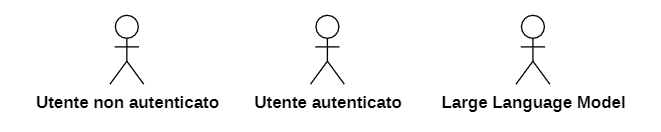
\includegraphics[width=1\textwidth]{usecase/attori.png}
    \caption{Attori dei casi d'uso}
    \label{fig:attori-casi-duso}
\end{figure}




\subsubsection{Casi d'uso individuati}
\label{subsubsec:casi-uso-individuati}

Descrizione dei casi d'uso individuati durante l'analisi dei requisiti.\\

\subsection{Tracciamento dei requisiti}
\label{subsec:requisiti}

Lista dei requisiti individuati, con spiegazione della notazione utilizzata e classificazione tra requisiti funzionali e non funzionali, obbligatori, desiderabili e facoltativi.\\